Na zmianę parametrów czujnika tensometrycznego metalowego największy wpływ ma wartość odkszałcenia
elementu, na którym zamontowany jest sensor. Jednakże istotną rolę dla pracy przetwornika stanowi
wpływ temperatury otoczenia. Aby zniwelować negatywny wpływ temperatury tensometry
pracują~w~układach mostkowych -- wyróżnia się układy ćwierćmostkowe, półmostkowe oraz pełnomostkowe,
przy czym tylko układy składające się~z~dwóch lub więcej tensometrów mają możliwość kompensacji
temperaturowej. Przykładowy schemat układu mostkowego przedstawiono na rysunku
\ref{img:strain-gauge}.

\begin{figure}[!htbp]
  \centering
  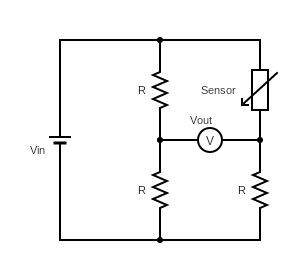
\includegraphics[width=0.5\textwidth]{sensor-theory/strain-quater}
  \caption{\label{img:strain-gauge}Przykładowy schemat układu mostkowego~z~tensometrami (tutaj:
    układ ćwierćmostkowy).}
\end{figure}

Zmianę rezystancji przetwornika tensometrycznego przedstawia zależność opisana wzorem
\ref{eq:strain-r}, natomiast~w~przypadku, gdy brany jest pod uwagę wpływ temperatury zależność ta
przedstawiona jest wzorem \ref{eq:strain-temp}. Wykonując pomiary naprężenia przetwornikami
tensometrycznymi, pracującymi~w~układzie mostkowym, należy mierzyć napięcie na wyjściu takiego
układu. Wykorzystując zależność przedstawioną równaniem \ref{eq:strain-bridge}, można wyznaczyć
teoretyczne napięcie wyjściowe układu.

\begin{equation}\label{eq:strain-r}
  \Delta R = R\cdot\varepsilon\cdot GF
\end{equation}

\begin{eqparams}
  R & bazowa rezystancja tensometru,\\
  \varepsilon & wartość odkształcenia,\\
  GF & współczynnik odkształcenia,\\
\end{eqparams}

\begin{equation}\label{eq:strain-temp}
  \Delta R = R(\varepsilon\cdot GF + \alpha\Delta T)
\end{equation}

\begin{eqparams}
  R & bazowa rezystancja tensometru,\\
  \varepsilon & wartość odkształcenia,\\
  GF & współczynnik odkształcenia,\\
  \alpha & współczynnik temperaturowy metalu (zgodnie~z~tabelą \ref{tab:temp_alpha}),\\
  \Delta T & różnica temperatur pomiędzy temperaturą otoczenia~a~odniesienia (20\degC),\\
\end{eqparams}

\begin{equation}\label{eq:strain-bridge}
  U_{wyj}=\frac{1}{4}\cdot U_{wej}\cdot\bigg(\frac{\Delta R_1}{R_1}-\frac{-\Delta R_2}{R_2}
  +\frac{\Delta R_3}{R_3}-\frac{-\Delta R_4}{R_4}\bigg)
\end{equation}

\begin{table}[!htbp]
  \begin{eqparams}
    R_i & bazowa rezystancja i-tego tensometru~w~mostku,\\
    \Delta R_i & zmiana rezystancji i-tego tensometru~w~mostku
    \tablefootnote{W zależności od typu mostka, jeżeli $R_i$ jest zwykłym rezystorem, to $\Delta R_i$ będzie równa 0.},\\
    U_{wej} & napięcie zasilania mostka,\\
  \end{eqparams}
\end{table}

